\documentclass[11pt,spanish,a4paper]{article}
% Versión 1.er cuat 2021 Víctor Bettachini < bettachini@df.uba.ar >

% Versión 1.er cuat 2021 Víctor Bettachini < bettachini@df.uba.ar >

\usepackage[T1]{fontenc}
\usepackage[utf8]{inputenc}

\usepackage[spanish, es-tabla]{babel}
\def\spanishoptions{argentina} % Was macht dass?
% \usepackage{babelbib}
% \selectbiblanguage{spanish}
% \addto\shorthandsspanish{\spanishdeactivate{~<>}}

\usepackage{graphicx}
\graphicspath{{./figuras/}}
% \usepackage{float}

\usepackage[arrowdel]{physics}
\newcommand{\pvec}[1]{\vec{#1}\mkern2mu\vphantom{#1}}
% \usepackage{units}
\usepackage[separate-uncertainty=true, multi-part-units=single, locale=FR]{siunitx}
\usepackage{isotope} % $\isotope[A][Z]{X}\to\isotope[A-4][Z-2]{Y}+\isotope[4][2]{\alpha}

\usepackage{tasks}
\usepackage[inline]{enumitem}
% \usepackage{enumerate}

\usepackage{hyperref}

% \usepackage{amsmath}
% \usepackage{amstext}
\usepackage{amssymb}

\usepackage{tikz}
\usepackage{tikz-dimline}
\usetikzlibrary{math}
\usetikzlibrary{arrows.meta}
% \usetikzlibrary{snakes}
% \usetikzlibrary{calc}
\usetikzlibrary{decorations.pathmorphing}
\usetikzlibrary{patterns}

\usepackage[hmargin=1cm,vmargin=1.6cm,nohead]{geometry}
% \voffset-3.5cm
% \hoffset-3cm
% \setlength{\textwidth}{17.5cm}
% \setlength{\textheight}{27cm}

\usepackage{lastpage}
\usepackage{fancyhdr}
\pagestyle{fancyplain}
\fancyhead{}
\fancyfoot{{\tiny \textcopyright DF, FCEyN, UBA}}
\fancyfoot[C]{ {\tiny Actualizado al \today} }
\fancyfoot[RO, LE]{Pág. \thepage/\pageref{LastPage}}
\renewcommand{\headrulewidth}{0pt}
\renewcommand{\footrulewidth}{0pt}


\begin{document}
\begin{center}
\textbf{Física 2} (Físicos) \hfill \textcopyright {\tt DF, FCEyN, UBA}\\
%	\textsc{\large Física 2 (Físicos)} - Prof. Diana Skigin - 2"o cuat. 2014\\
%	\textsc{\large Primer Cuatrimestre - 2014}\\
	\textsc{\LARGE Sistemas con dos grados de libertad}
	% \textsc{\large Guía 1:} Oscilaciones libres y forzadas
\end{center}

Los ejercicios con (*) son opcionales.

\begin{enumerate}


\item Asuma que el sistema de la figura no está bajo el efecto de un campo gravitatorio
\begin{figure}[h]
	\centering
	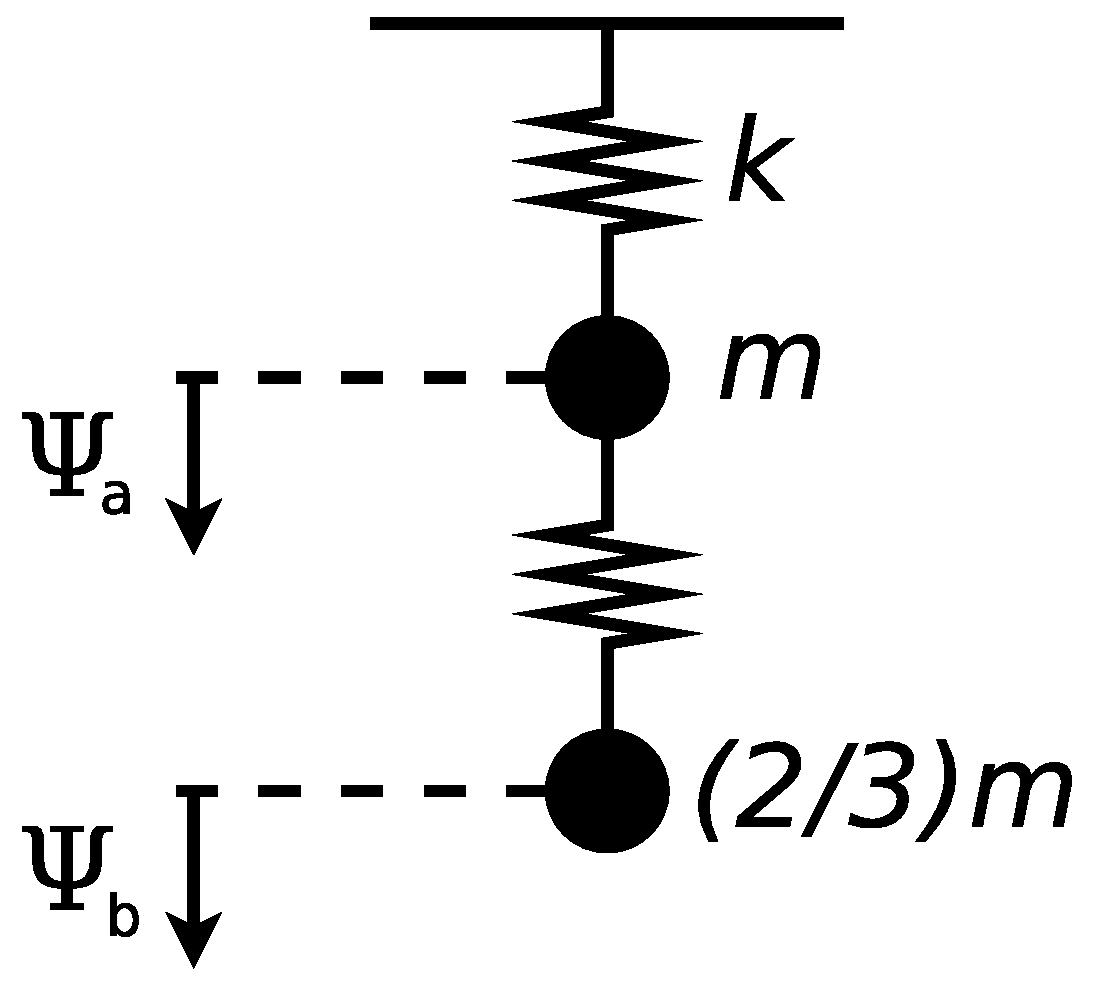
\includegraphics[clip,scale=0.25]{ej1-6}
\end{figure}
\begin{enumerate}
	% \item Considere el sistema de la figura en ausencia de gravedad y obtenga sus frecuencias naturales de oscilación y los modos normales correspondientes.
	\item Obtenga sus frecuencias naturales de oscilación y los modos normales correspondientes.
	Escriba las ecuaciones de movimiento de cada partícula.
	\item Sabiendo que a $t= 0$ el sistema satisface las siguientes condiciones: $\Psi_a(0)= 1, \, \Psi_b(0)= 0$ y que se encuentra en reposo, encuentre el movimiento de cada partícula.
	\item Analice cómo se modifica el resultado por la presencia de la gravedad en la superficie de la Tierra.
\end{enumerate}



\item En el sistema de la figura se tienen dos partículas de masa $m$ unidas a las paredes con resortes dispuestos verticalmente de longitud natural $l_0$ ($l_0< L/2$) y constante elástica $k_1$, y con otros dispuestos horizontontalmente de $l_0= 0$ (\emph{slinkies}) y constante $k_2$.
Imagine que las partículas tienen la libertad de moverse en el plano y que el sistema no está en un campo gravitatorio.
\begin{figure}[h]
	\centering
	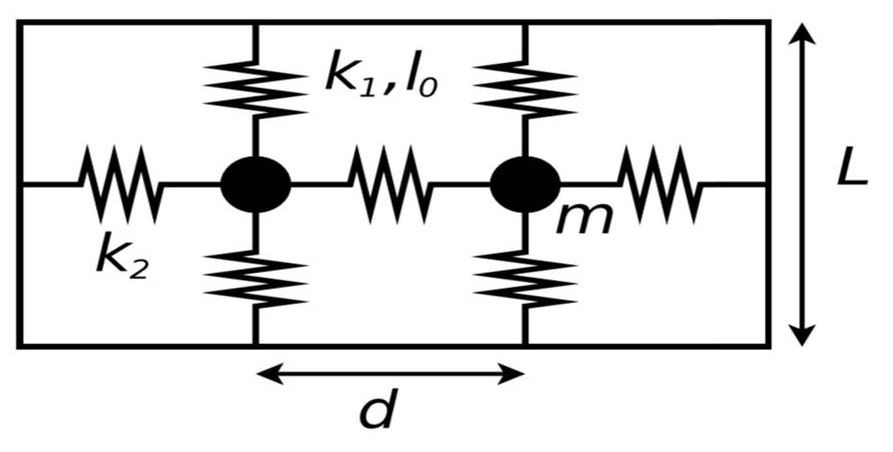
\includegraphics[clip,scale=0.45]{resortes_acoplados}
\end{figure}
\begin{enumerate}
    \item ¿Bajo qué aproximaciones es posible decir que el movimiento más general posible de cada una de las masas es una superposición lineal del movimiento más general posible de las oscilaciones longitudinales y de las oscilaciones transversales?
		Demuestre su afirmación.
    \item Considerando la aproximación del punto anterior, determine las frecuencias propias y los modos normales de oscilación: longitudinales, transversales y de la solución más general posible para un movimiento arbitrario en el plano.
\end{enumerate}



\item \label{pendacop} De dos péndulos de igual longitud $l$ penden pesos de masas diferente $m_a$ y $m_b$.
Estas están acopladas entre sí mediante un resorte de constante elástica $k$.
\begin{figure}[h]
	\centering
	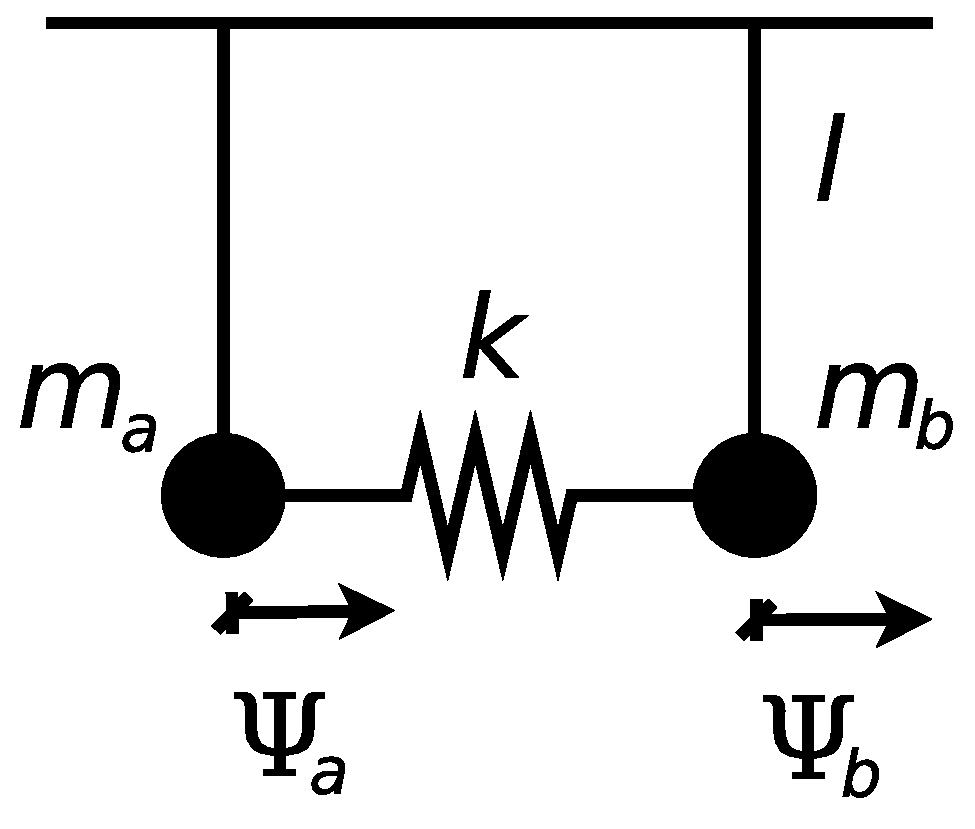
\includegraphics[clip,scale=0.3]{ej1-7}
\end{figure}
\begin{enumerate}
	\item Escriba las ecuaciones de movimiento de cada masa. considerando pequeñas oscilaciones, ¿es relevante considerar $l_0 \neq 0$?
	¿Qué cambia si el resorte es \emph{slinky}?   
	\item Obtenga las frecuencias naturales del sistema y sus modos normales de oscilación.
	Interprete el significado físico de estos modos normales. 
\end{enumerate}


\item \label{2masitas} Dos pesas de idéntica masa están apoyadas en una mesa sin rozamiento, sujetas a las paredes por resortes de constante
elástica $k$ y unidas entre sí por otro con distianta constante $k'$.
Obtenga las frecuencias y los modos transversales del sistema. 
\begin{figure}[h]
	\centering
	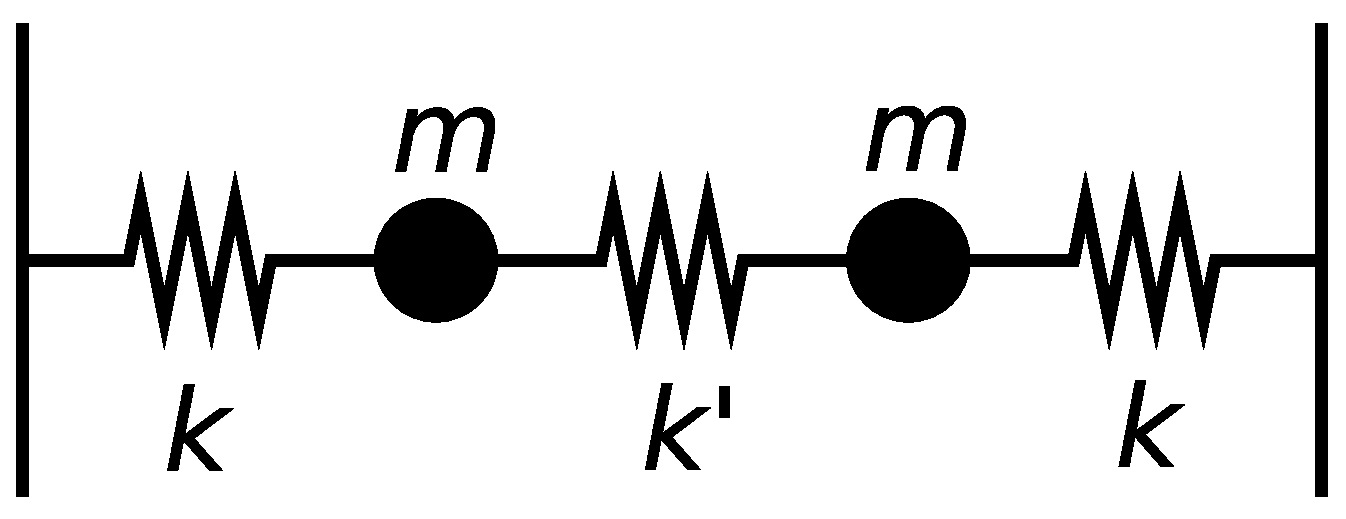
\includegraphics[clip,scale=0.25]{ej1-8}
\end{figure}



\subsection*{Sistemas forzados}
\item Considere el sistema de dos péndulos acoplados del problema \ref{pendacop}, tal que uno de ellos es impulsado por una fuerza $F= F_0 \cos(\Omega t)$.  
\begin{enumerate}
	\item Escriba las ecuaciones de movimiento del sistema con amortiguamiento y forzado y desacople las ecuaciones utilizando las coordenadas normales del sistema.
	\item Resuelva el sistema forzado para las coordenadas normales y luego escriba la solución más general posible para las coordenadas de las partículas a y b.
	\item Estudie el caso estacionario, observe cuando las partículas están en fase o contrafase.
	\item Muestre que considerando $m_a= m_b= m$ y despreciando el amortiguamiento se obtienen las siguientes expresiones.
		\begin{align}
			\Psi_a &\approx \frac{F_0}{2m} \cos(\Omega t) \left[ \frac{1}{\omega_1^2 - \Omega^2 } + \frac{1}{\omega_2^2 -\Omega^2} \right] \notag \\
			\Psi_b &\approx \frac{F_0}{2m} \cos(\Omega t) \left[ \frac{1}{\omega_1^2 - \Omega^2 } - \frac{1}{\omega_2^2 -\Omega^2} \right] \notag \\
			\frac{\Psi_b}{\Psi_a} &\approx \frac{\omega_2^2 - \omega_1^2}{\omega_2^2 + \omega_1^2 - 2 \Omega^2} \notag
		\end{align}
	donde $\omega_{1}$ es la menor de las frecuencias modales, $\omega_{2}$ es la mayor y $\Omega$ es la frecuencia de excitación.
	\item (*) Grafique $\frac{\Psi_b}{\Psi_a}$, ¿qué representa esta relación?
	Indique cuándo hay una transferencia efectiva de movimiento y cuándo no.
\end{enumerate}


\item Considere el sistema del problema \ref{2masitas}, pero en este caso en considere las oscilaciones longitudinales.
\begin{enumerate}
    \item Halle la solución estacionaria para el caso forzado en el cual se aplica sobre la masa de la izquierda una fuerza oscilante $F(t)= F_0 cos(\Omega t)$.
		¿Qué resonancias espera ver si realiza un barrido de frecuencias?
		\item (*) Repita el punto anterior, teniendo en cuenta además una fuerza de disipación proporcional a la velocidad
		\item (*) Repita el problema pero considerando las oscilaciones transversales del sistema
\end{enumerate}


\end{enumerate}

\end{document}
